\section{RFC-0007: Economic Reward
System}\label{rfc-0007-economic-reward-system}

\begin{itemize}
\tightlist
\item
  \textbf{RFC Number:} 0007
\item
  \textbf{Title:} Economic Reward System
\item
  \textbf{Status:} Raw
\item
  \textbf{Author(s):} Jean Demeusy (@jeandemeusy)
\item
  \textbf{Created:} 2025-08-25
\item
  \textbf{Updated:} 2025-08-25
\item
  \textbf{Version:} v0.1.0
\item
  \textbf{Supersedes:} N/A
\item
  \textbf{Related Links:} none
\end{itemize}

\subsection{1. Abstract}\label{1-abstract}

This RFC describes mechanisms around the economic reward system such as
how the eligible peer set is constructed and how the rewards per peer
are calculated

\subsection{2. Motivation}\label{2-motivation}

The rewards calculation can be seen as an opaque procedure selecting who
receives which amount. This RFC aims to raise the veil and clarify the
reasoning behind it.

The economic reward system is a necessary component of the HOPR mixnet,
as it incentivize node runners to keep their node running, in order to
have a network topology as stable as possible. It must be a fair logic,
to never favour or disadvantage a subset of node runners, that
encourages sustainability without compromising decentralization. It must
also incentivize node runners to be connected to other nodes in the
network with channels. Isolated nodes are way less useful to the network
than well intricately connected nodes.

\subsection{3. Terminology}\label{3-terminology}

\begin{itemize}
\tightlist
\item
  \textbf{Subgraph}: Off-chain data indexer (e.g., The Graph) for
  blockchain data (NFT holders, registered nodes, allocations, EOA
  balances).
\item
  \textbf{API}: HOPR node HTTP API for live network data (topology,
  channel balances).
\item
  \textbf{EOA (Externally Owned Account)}: Blockchain account controlled
  by a private key.
\item
  \textbf{Safe}: Smart contract wallet (e.g., Gnosis Safe) for holding
  tokens.
\item
  \textbf{CT Node}: Node running the CT application.
\item
  \textbf{NFT Holder}: Address holding a specific NFT.
\item
  \textbf{SessionToSocket}: Object managing a UDP session and socket for
  a peer.
\item
  \textbf{MessageFormat}: Class encoding message metadata and payload as
  bytes.
\end{itemize}

The key words "MUST", "MUST NOT", "REQUIRED", "SHALL", "SHALL NOT",
"SHOULD", "SHOULD NOT", "RECOMMENDED", "MAY", and "OPTIONAL" in this
document are to be interpreted as described in
\href{https://datatracker.ietf.org/doc/html/rfc2119}{IETF RFC 2119}.

\subsection{4. System Overview}\label{4-system-overview}

The HOPR CT system is designed to distribute rewards to eligible peers
based on their participation and stake in the network. The process is
composed of several key stages. First, the system collects and enriches
peer data from a variety of sources, including both on-chain and
off-chain information. Next, it applies a series of eligibility filters
to determine which peers qualify for rewards. For those that are
eligible, an economic model is used to calculate the number of reward
units (messages) each peer should receive. Finally, the system manages
the technical process of sending these messages to peers using UDP
sessions, ensuring that the distribution is both fair and technically
robust.

The following flowchart summarizes the overall process:

\pandocbounded{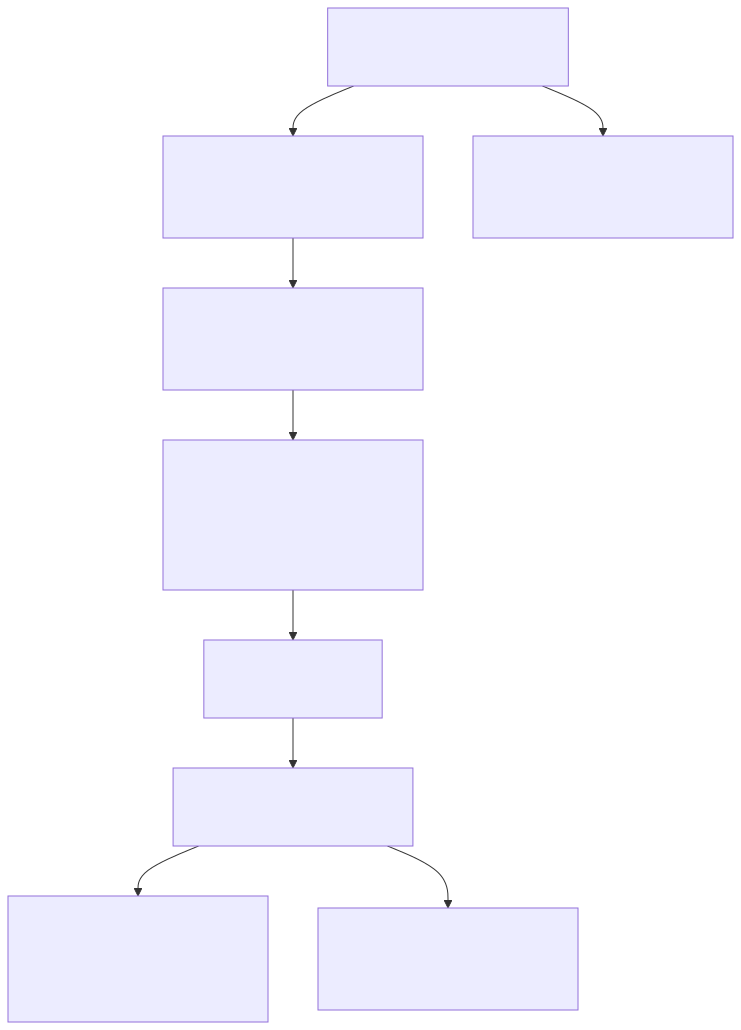
\includegraphics[keepaspectratio,width=\maxwidth,alt={Mermaid Diagram 1}]{generated/0007-economic-reward-system/mermaid_1.png}}

\subsection{5. Data Collection and
Enrichment}\label{5-data-collection-and-enrichment}

\subsubsection{5.1 Data Sources}\label{51-data-sources}

Data is gathered from multiple sources to build a comprehensive view of
the network and its participants. The HOPR node API provides a list of
currently visible peers and the network topology, including open payment
channels and their balances. Subgraphs supply information about
registered nodes and their associated Safes. Direct RPC calls are used
to provide specific allocations to targeted accounts (which may increase
a peer\textquotesingle s effective stake) and to retrieve those
accounts\textquotesingle{} EOA balances. Finally, a static list of NFT
owners is used to allow rewards distribution to people holding a special
``OG NFT''. This combination of sources ensures that both the live state
of the network and relevant historical or off-chain data are considered
in the reward process.

\subsubsection{5.2 Data Enrichment}\label{52-data-enrichment}

Once collected, the data is used to enrich each peer object. Registered
node information is used to associate each peer with a Gnosis Safe and
other node metadata. Allocations and EOA balances are incorporated to
adjust the peer\textquotesingle s effective stake and balance,
reflecting both on-chain and off-chain holdings. The network topology
data is used to determine the peer\textquotesingle s channel balance,
which is important for both eligibility and reward calculation. It is
important to note that NFT holder status and CT node status are not
directly added to the peer object during enrichment; instead, these are
checked during the eligibility filtering phase.

The following diagram illustrates the data enrichment process:

\pandocbounded{\includegraphics[keepaspectratio,width=\maxwidth,alt={Mermaid Diagram 2}]{generated/0007-economic-reward-system/mermaid_2.png}}

\subsection{6. Peer Eligibility
Filtering}\label{6-peer-eligibility-filtering}

The eligibility filtering process is designed to ensure that only peers
who are meaningfully participating in the network and contributing
resources are considered for rewards. The first filter checks that the
peer\textquotesingle s safe allowance meets a minimum threshold,
ensuring that only active and funded peers are included. Next, the
system excludes any peer that is also a CT node, to prevent
self-rewarding. The NFT/stake requirement is then applied: if a peer is
not an NFT holder, they must meet a higher minimum stake threshold,
while NFT holders may be subject to a lower threshold. Finally, all
peers must meet a minimum stake requirement, regardless of NFT status.
Only those who pass all these checks are considered eligible for
rewards.

The following flowchart details the filtering logic:

\pandocbounded{\includegraphics[keepaspectratio,width=\maxwidth,alt={Mermaid Diagram 3}]{generated/0007-economic-reward-system/mermaid_3.png}}

\subsection{7. Economic Model
Application}\label{7-economic-model-application}

For each eligible peer, the system applies an economic model---such as a
sigmoid or legacy model---to determine the number of messages (reward
units) they should receive over the course of a year. The model takes
into account the peer\textquotesingle s individual stake, the total
network stake, the network\textquotesingle s capacity, and historical
activity metrics such as message relay counts. The output of this model
is the yearly message count for each peer, which directly determines
their share of the rewards.

The following diagram shows the economic model application:

\pandocbounded{\includegraphics[keepaspectratio,width=\maxwidth,alt={Mermaid Diagram 4}]{generated/0007-economic-reward-system/mermaid_4.png}}

\subsection{8. Message Timing and Delay
Calculation}\label{8-message-timing-and-delay-calculation}

The timing between messages sent to each eligible peer is carefully
calculated to ensure a fair and even distribution throughout the year.
The base delay between two messages is computed as the total number of
seconds in a non-leap year divided by the peer\textquotesingle s yearly
message count. To allow for efficient batching and aggregation, the
system introduces two session parameters: \texttt{aggregated\_packets}
and \texttt{batch\_size}. The actual sleep time between message batches
is the product of the base delay, the number of aggregated packets, and
the batch size. This approach allows the system to send bursts of
messages followed by a pause, balancing throughput and network load. The
values of these parameters can be tuned to optimize performance and
reliability.

The \texttt{aggregated\_packets} parameter specifies how many messages
are grouped together and sent in a single relay operation, while
\texttt{batch\_size} determines how many such operations are performed
before the system waits for the next delay interval. The product of
these two parameters gives the total number of messages sent in each
cycle, and the delay is applied after each cycle. This mechanism
provides fine-grained control over the message sending pattern.

\subsection{9. Message Sending
Architecture}\label{9-message-sending-architecture}

When it is time to send messages, the system first establishes a UDP
session for each eligible peer, selecting a destination CT node at
random (excluding the local node). Each session is managed by a
\texttt{SessionToSocket} object, which handles both the session metadata
and the underlying UDP socket. The socket is configured with appropriate
buffer sizes and is closed when the session ends to prevent resource
leaks.

Messages themselves are constructed using the \texttt{MessageFormat}
class, which encodes all necessary metadata---such as sender, relayer,
packet size, and indices---into a raw byte string. The message is padded
to the required packet size and sent through the UDP socket to the
destination node\textquotesingle s address and port. The system can
optionally wait for a response to measure round-trip time, which is
useful for monitoring and diagnostics.

Batching multiple message sendings are handled according to the session
parameters described earlier. Multiple messages can be sent in a batch,
and after each batch, the system waits for the calculated delay before
sending the next batch. This approach ensures that message delivery is
both efficient and aligned with the reward allocation determined by the
economic model.

The following flowchart summarizes the message sending process:

\pandocbounded{\includegraphics[keepaspectratio,width=\maxwidth,alt={Mermaid Diagram 5}]{generated/0007-economic-reward-system/mermaid_5.png}}

\subsection{10. Security and
Monitoring}\label{10-security-and-monitoring}

Security and monitoring are integral to the HOPR CT reward distribution
process. To ensure transparency and facilitate troubleshooting, all
delays and message counts are tracked using Prometheus metrics. This
allows operators and developers to monitor the system\textquotesingle s
performance in real time, detect anomalies, and analyze historical
trends.

Resource management is also a key concern. The system is designed to
manage sessions and sockets carefully, ensuring that resources are
allocated and released appropriately. Sockets are closed when sessions
end, and sessions are only maintained for as long as they are needed.
This approach helps prevent resource leaks, which could otherwise
degrade system performance or cause failures over time.

Finally, the system enforces strict eligibility checks before sending
messages. Only peers that have open payment channels and valid, active
sessions are eligible to receive messages. This ensures that rewards are
distributed only to those who are actively participating in the network
and have met all necessary criteria, further enhancing the security and
integrity of the reward process.

\subsection{11. Appendix: Data
Structures}\label{11-appendix-data-structures}

\subsubsection{Registered Node}\label{registered-node}

\begin{longtable}[]{@{}lll@{}}
\toprule\noalign{}
Variable Name & Type & Purpose \\
\midrule\noalign{}
\endhead
\bottomrule\noalign{}
\endlastfoot
address & str & Node\textquotesingle s unique address \\
safe & Safe & Associated Gnosis Safe object \\
... & ... & (Other metadata as provided by subgraph) \\
\end{longtable}

\subsubsection{Safe}\label{safe}

\begin{longtable}[]{@{}lll@{}}
\toprule\noalign{}
Variable Name & Type & Purpose \\
\midrule\noalign{}
\endhead
\bottomrule\noalign{}
\endlastfoot
address & str & Safe contract address \\
balance & Balance & Total balance held in the safe \\
allowance & Balance & Allowance available for node operations \\
additional\_balance & Balance & Extra balance from allocations/EOA \\
owners & list & List of owner addresses \\
... & ... & (Other metadata as provided by subgraph) \\
\end{longtable}

\subsubsection{Allocation}\label{allocation}

\begin{longtable}[]{@{}lll@{}}
\toprule\noalign{}
Variable Name & Type & Purpose \\
\midrule\noalign{}
\endhead
\bottomrule\noalign{}
\endlastfoot
address & str & Allocation contract address \\
unclaimed\_amount & Balance & Amount not yet claimed \\
linked\_safes & set & Safes associated with this allocation \\
num\_linked\_safes & int & Number of safes linked \\
\end{longtable}

\subsubsection{EOA Balance}\label{eoa-balance}

\begin{longtable}[]{@{}lll@{}}
\toprule\noalign{}
Variable Name & Type & Purpose \\
\midrule\noalign{}
\endhead
\bottomrule\noalign{}
\endlastfoot
address & str & EOA address \\
balance & Balance & Balance held by the EOA \\
linked\_safes & set & Safes associated with this EOA \\
num\_linked\_safes & int & Number of safes linked \\
\end{longtable}

\subsubsection{Topology Entry}\label{topology-entry}

\begin{longtable}[]{@{}lll@{}}
\toprule\noalign{}
Variable Name & Type & Purpose \\
\midrule\noalign{}
\endhead
\bottomrule\noalign{}
\endlastfoot
address & str & Peer address \\
channels\_balance & Balance & Total balance in outgoing channels \\
\end{longtable}

\subsubsection{Peer (Enriched)}\label{peer-enriched}

\begin{longtable}[]{@{}lll@{}}
\toprule\noalign{}
Variable Name & Type & Purpose \\
\midrule\noalign{}
\endhead
\bottomrule\noalign{}
\endlastfoot
address & Address & Peer's unique address \\
version & Version & Peer's software version \\
safe & Safe & Associated safe object \\
channel\_balance & Balance & Balance in outgoing channels \\
yearly\_message\_count & int/None & Calculated reward allocation \\
params & Parameters & Application parameters \\
running & bool & Is the peer currently active \\
... & ... & (Other runtime attributes) \\
\end{longtable}

\subsection{12. References}\label{12-references}

None.

\subsection{13. Changelog}\label{13-changelog}

\begin{itemize}
\tightlist
\item
  2025-06-26: Initial draft.
\end{itemize}
